% !TeX spellcheck = en_US
\documentclass[11pt, fleqn, titlepage]{article}
%\usepackage{siunitx}
\usepackage{texfiles/SpeedyGonzales}
\usepackage{texfiles/MediocreMike}
\newcommand{\so}[2]{{#1}\mathrm{e}{#2}}
% \geometry{top=1cm}
\usepackage{hyperref}
\usepackage{amsmath}
\usepackage{ragged2e}
\usepackage{booktabs}
\hypersetup{
	colorlinks=true,
	linkcolor=blue,
	filecolor=magenta,      
	urlcolor=cyan,
}
\usepackage{subfig}
\usepackage{graphicx}
\title{Fairness in Classification}
\author{Oskar Eiler Wiese Christensen s183917 \\ Anders Henriksen s183904}
\date{\today}
	

\pagestyle{plain}
\fancyhf{}
\rfoot{Page \thepage{} of \pageref{LastPage}}

\graphicspath{{Billeder/}}

\begin{document}
	
	\maketitle
	\tableofcontents \newpage
	%\thispagestyle{fancy}
	%\tableofcontents
	\section{Abstract}
	
	
	\section{Introduction}
	
	
	
	\section{Data}
	
	\subsection{Description of Data}
	The data used in this project stems from an initial analysis of the COMPAS (Correctional Offender Management Profiling for Alternative Sanctions) algorithm by its developers, Northpointe Inc. After this analysis, ProPublica made a subsequent analysis of this data as well as their own queries of the offenders involved and data of the offenders who actually recidivated. This data is stored in the \texttt{compas-scores-two-year.csv} dataset from ProPublica's GitHub page, which can be found here: \url{https://github.com/propublica/compas-analysis/blob/master/compas-scores-two-years.csv}. \\\\
	\noindent The data consists of 53 different variables, 9 of which are used in the binary classification model. Four of the chosen variables are categorical, so these will have to be one-out-of-k encoded to be able to feed the necessary variables into the neural network. Meanwhile, the numerical variables, of which there are also four, will be normalized as to avoid the vanishing gradient problem and to avoid having some variables be of more importance to the final prediction. This will be explained more thoroughly in \ref{Feed-forward neural}. \\
	The 10 chosen variables, of which one will be used as the target variable are shown and explained below.
	
	
	\begin{table}[H]\label{resultater}
		\centering
		\begin{tabular}{l l l}
			Variable & Description & Type \\ \hline
			age & The age of the offenders & Continuous ratio \\
			priors\_count & The number of previous offences & Discrete interval \\
			juv\_fel\_count & The number of previous juvenile felonies & Discrete interval \\
			juv\_misd\_count & The number of previous juvenile misdemeanor & Discrete interval \\
			c\_charge\_degree & The severity of the offence & Discrete nominal \\
			race & The race of the offender & Discrete nominal \\
			age\_cat & The age category of the offender & Discrete nominal \\
			sex & The sex of the offender & Discrete nominal \\
			score\_text & The COMPAS prediction of chance of recidivism & Discrete interval
		\end{tabular}
		%\caption{text}
	\end{table}
		
		
	\subsection{Visualization of Data}
		
		
	\subsection{Bias in Data}
		
		
	\section{Methods}
	 
	\subsection{Binary Classifier}\label{Feed-forward neural}
	%initialization schemes
	\subsubsection{Feed-forward Neural Network}
	Feed-forward neural networks (FFNN) are the simplest form of a neural network. Information flow in a feed-forward neural is one directional which means that the network has an input layer, and information flow from these nodes through the hidden layers unto the output layer. The main purpose of a FFNN is to approximate a function. In this project $ y = f^*(x) $ maps an input $ \mathbf x $ to a category $ \mathbf y $. The FFNN is thereby a classifier, which goal is to determine the recidvism risk of a person given the input variable $ \mathbf x $. The input variable $ \mathbf x $ contains :::::. The categories of $ \mathbf y $ is either 0 or 1, which corresponds to the classifier classifying a person as either low or medium/high risk of recidivism. Hence, this is a binary classifier which constructs a mapping $ \mathbf y = f(\mathbf x \ ; \mathbf w) $. The goal is to learn the weights that most efficiently approximate the function $ f^* $ through supervised learning. The binary classifier in this project has an input layer, three hidden layers and an output layer. 
	
	\begin{figure}[H]
		\centering
		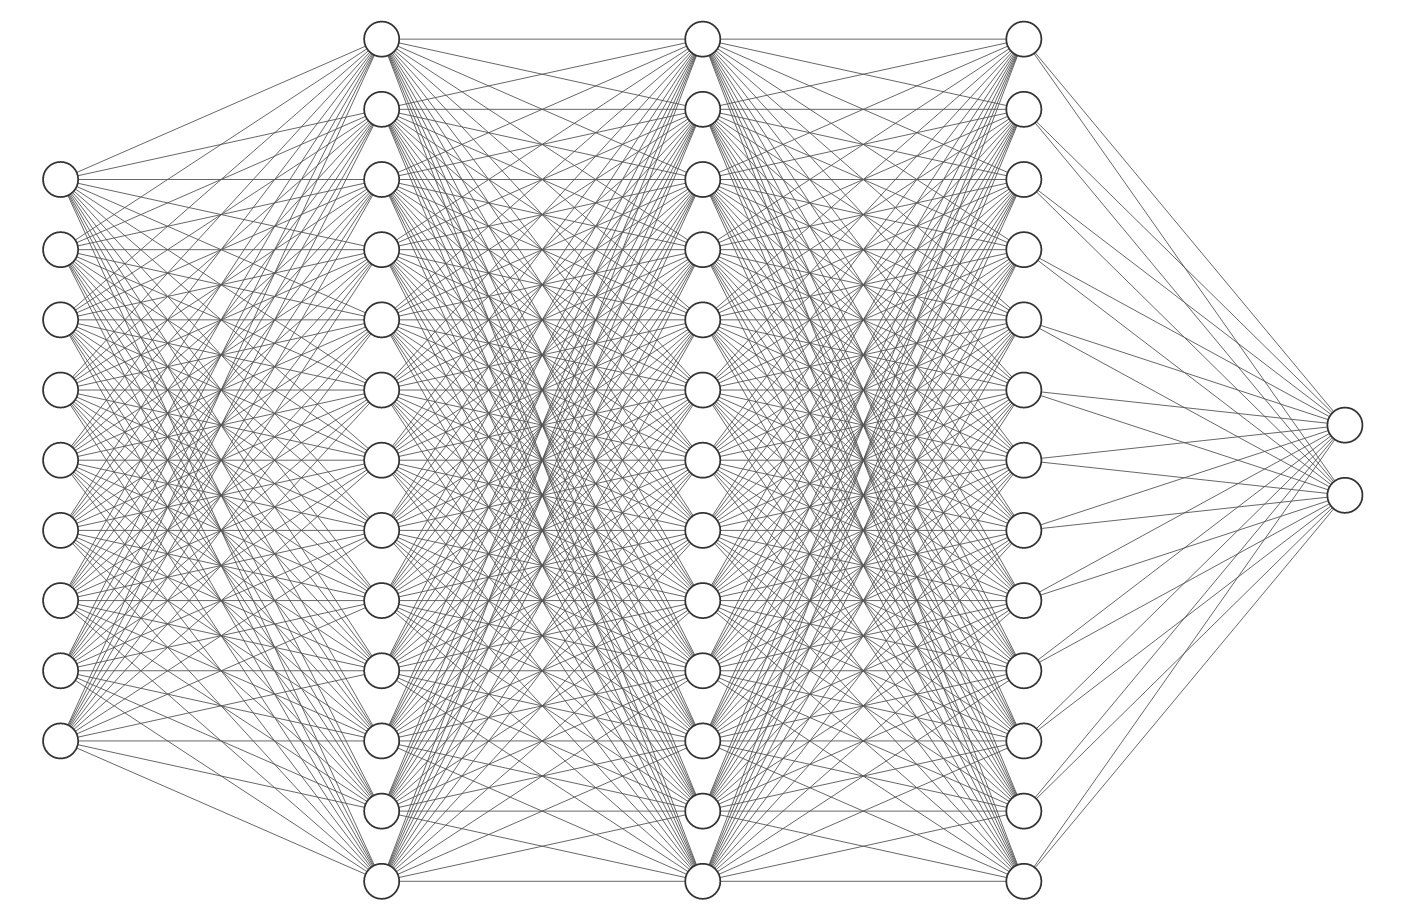
\includegraphics[width=0.5\linewidth]{imgs/ffnn}
		\caption{Visualization of the binary classifier model. The input layer has dimension $ \mathbb R ^9$ and the output layer has dimension $ \mathbb R^2 $. The number of nodes in the hidden layers is a changeable parameter which is found with Bayesian Optimization. }
		\label{fig:ffnn}
	\end{figure}
	
	
	\subsubsection{Bayesian Optimization}
	%Bayesian Optimization
	
	To obtain the pinnacle of accuracy in a neural network, it needs an excellent architecture as well as the potimal hyperparameters. However, the search for these parameters are usually a costly process of uncertainty balancing exploration of parameters and the exploitation of results. Often the process of finding the optimal parameters and network architecture comes from expert knowledge, biased heuristics or exhaustive sampling from the parameter space. To determine the architecture and hyperparameters of the binary classifier Bayesian Optimization is used. 
	\subparagraph*{Objective Function}
	The objective function that is being optimized in this project is the binary classifier presented above. The fully connected layers are trained on the COMPASS data-set and the validation accuracy of the model is what BO optimizes. The accuracy of the constructed model is evaluated using non-parametric Gaussian Process (GP) as a function fo the following hyperparameters:
	\begin{itemize}
		\item Number of units in the first hidden layer \(\in [1, 5000]\) 
		\item Number of units in the second hidden layer \(\in [1, 5000]\) 
		\item Number of units in the third hidden layer \(\in [1, 5000]\)
		\item Dropout probability \(\in [0,1]\)
		\item Activation function \{tanh, ReLU, ReLU6, Sigmoid\}
	\end{itemize}
	The hyperparameters that are not changed are the learning rate, which is set at $ \alpha = 0.001 $. The reason why this parameter is not changed is due to the fact, that the optimizer implemented in this project, is Adaptive Moment Estimation (Adam). Adam is a well known optimizer in the literature and has adaptive learning rate as well as step size. Which is why this learning rate is not an interchangeable hyperparameter. \\ Cross Entropy Loss is used as the cost-function. \textbf{TODO: skriv noget om funktionen. }
	\\\\
	Gaussian Process uses the smoothness assumption on the outputs of the network, and its variance and lengthscale parameters are optimized using maximum log-likelihood principle. \cite{aktiv_gp} The acquisition function, that choose the parameters for the model, used is Expected Improvement (EI). EI attempts to quantify the improvement of the parameters chosen. The average improvement is quantified by sampling the objective function at $x$. The acquisition function then computes the expected value of the improvement function at a certain $x$. EI is expressed as 
	\begin{equation*}
	\mathrm{EI}(\mathbf{x})=\left\{\begin{array}{ll}
	\left(\mu(\mathbf{x})-f\left(\mathbf{x}^{+}\right)\right) \Phi(Z)+\sigma(\mathbf{x}) \phi(Z) & \text { if } \sigma(\mathbf{x})>0 \\
	0 & \text { if } \sigma(\mathbf{x})<0,
	\end{array}\right. 
	\end{equation*}
	where $ Z = \frac{\mu(\mathbf{x}) - f(\mathbf{x}^+) - \xi }{\sigma(\mathbf{x})}$ , \cite{aktiv_bo} 
	\\\\
	The Bayesian Optimization starts by sampling from the objective function, then it fits the Gaussian Process to the sampled points and then iterates the next points in the hyperparameter space using the fitted GP and Expected Improvement. As for the implementation of Baysesian Optimization the GPyOpt library is used \cite{bo_lib}. The exploration / exploitation trade-off variable \textit{jitter} is set to the default value of 0.01.
	
	\subsection{Permutation test}
	
	\subsection{Bias Correction Methods}
	
	\section{Results}
	
	
	\section{Discussion}
	
	
	\section{Conclusion}
	
	\newpage
	\bibliographystyle{IEEEbib}
	\bibliography{refs}
\end{document}
